%\documentclass[AER]{AEA}
\documentclass[12pt]{report}
%\documentclass[12pt]{article}
%\documentclass[12pt,a4paper]{article}

\usepackage[utf8]{inputenc}


\usepackage{mathtools}
\usepackage{amsmath}
\usepackage{amssymb}
\usepackage{amsthm}

\usepackage{float}
%\usepackage[cmbold]{mathtime}
%\usepackage{mt11p}
\usepackage{placeins}
\usepackage{caption}
\usepackage{color}
\usepackage{subfigure}
\usepackage{multirow}
\usepackage{epsfig}
\usepackage{listings}
\usepackage{enumitem}
\usepackage{rotating,tabularx}
%\usepackage[graphicx]{realboxes}
\usepackage{graphicx}
\usepackage{graphics}
\usepackage{epstopdf}
\usepackage{longtable}

\usepackage{hyperref}

%\usepackage{breakurl}
\usepackage{epigraph}
\usepackage{xspace}
\usepackage{amsfonts}
\usepackage{eurosym}
\usepackage{ulem}

\usepackage{tikz}
\usetikzlibrary{spy}

\usepackage{verbatim}



\usepackage{footmisc}
\usepackage{comment}
\usepackage{setspace}
\usepackage{geometry}
\usepackage{caption}
\usepackage{pdflscape}
\usepackage{array}
\usepackage[authoryear]{natbib}
\usepackage{booktabs}
\usepackage{dcolumn}
\usepackage{mathrsfs}
%\usepackage[justification=centering]{caption}
%\captionsetup[table]{format=plain,labelformat=simple,labelsep=period,singlelinecheck=true}%
\bibliographystyle{apalike}
%\bibliographystyle{unsrtnat}



%\bibliographystyle{aea}
\usepackage{enumitem}
\usepackage{tikz}
\usetikzlibrary{positioning}
\usetikzlibrary{arrows}
\usetikzlibrary{shapes.multipart}

\usetikzlibrary{shapes}
\def\checkmark{\tikz\fill[scale=0.4](0,.35) -- (.25,0) -- (1,.7) -- (.25,.15) -- cycle;}
%\usepackage{tikz}
%\usetikzlibrary{snakes}
%\usetikzlibrary{patterns}

%\draftSpacing{1.5}

\usepackage{xcolor}
\hypersetup{
colorlinks,
linkcolor={blue!50!black},
citecolor={blue!50!black},
urlcolor={blue!50!black}}

%\renewcommand{\familydefault}{\sfdefault}
%\usepackage{helvet}
%\setlength{\parindent}{0.4cm}
%\setlength{\parindent}{2em}
%\setlength{\parskip}{1em}

%\normalem

%\doublespacing
\onehalfspacing
%\singlespacing
%\linespread{1.5}

\newtheorem{theorem}{Theorem}
\newtheorem{corollary}[theorem]{Corollary}
\newtheorem{proposition}{Proposition}
\newtheorem{definition}{Definition}
\newtheorem{axiom}{Axiom}
\newtheorem{observation}{Observation}
\newtheorem{assumption}{Assumption}	
\newtheorem{remark}{Remark}
\newtheorem{lemma}{Lemma}
\newtheorem{result}{result}


\newcommand{\ra}[1]{\renewcommand{\arraystretch}{#1}}

\newcommand{\E}{\mathrm{E}}
\newcommand{\Var}{\mathrm{Var}}
\newcommand{\Corr}{\mathrm{Corr}}
\newcommand{\Cov}{\mathrm{Cov}}

\newcolumntype{d}[1]{D{.}{.}{#1}} % "decimal" column type
\renewcommand{\ast}{{}^{\textstyle *}} % for raised "asterisks"

\newtheorem{hyp}{Hypothesis}
\newtheorem{subhyp}{Hypothesis}[hyp]
\renewcommand{\thesubhyp}{\thehyp\alph{subhyp}}

\newcommand{\red}[1]{{\color{red} #1}}
\newcommand{\blue}[1]{{\color{blue} #1}}

%\newcommand*{\qed}{\hfill\ensuremath{\blacksquare}}%

\newcolumntype{L}[1]{>{\raggedright\let\newline\\arraybackslash\hspace{0pt}}m{#1}}
\newcolumntype{C}[1]{>{\centering\let\newline\\arraybackslash\hspace{0pt}}m{#1}}
\newcolumntype{R}[1]{>{\raggedleft\let\newline\\arraybackslash\hspace{0pt}}m{#1}}

%\geometry{left=1.5in,right=1.5in,top=1.5in,bottom=1.5in}
\geometry{left=1in,right=1in,top=1in,bottom=1in}

\epstopdfsetup{outdir=./}

\newcommand{\elabel}[1]{\label{eq:#1}}
\newcommand{\eref}[1]{Eq.~(\ref{eq:#1})}
\newcommand{\ceref}[2]{(\ref{eq:#1}#2)}
\newcommand{\Eref}[1]{Equation~(\ref{eq:#1})}
\newcommand{\erefs}[2]{Eqs.~(\ref{eq:#1}--\ref{eq:#2})}

\newcommand{\Sref}[1]{Section~\ref{sec:#1}}
\newcommand{\sref}[1]{Sec.~\ref{sec:#1}}

\newcommand{\Pref}[1]{Proposition~\ref{prop:#1}}
\newcommand{\pref}[1]{Prop.~\ref{prop:#1}}
\newcommand{\preflong}[1]{proposition~\ref{prop:#1}}

\newcommand{\Aref}[1]{Axiom~\ref{ax:#1}}

\newcommand{\clabel}[1]{\label{coro:#1}}
\newcommand{\Cref}[1]{Corollary~\ref{coro:#1}}
\newcommand{\cref}[1]{Cor.~\ref{coro:#1}}
\newcommand{\creflong}[1]{corollary~\ref{coro:#1}}

\newcommand{\etal}{{\it et~al.}\xspace}
\newcommand{\ie}{{\it i.e.}\ }
\newcommand{\eg}{{\it e.g.}\ }
\newcommand{\etc}{{\it etc.}\ }
\newcommand{\cf}{{\it c.f.}\ }
\newcommand{\ave}[1]{\left\langle#1 \right\rangle}
\newcommand{\person}[1]{{\it \sc #1}}

\newcommand{\AAA}[1]{\red{{\it AA: #1 AA}}}
\newcommand{\YB}[1]{\blue{{\it YB: #1 YB}}}

\newcommand{\flabel}[1]{\label{fig:#1}}
\newcommand{\fref}[1]{Fig.~\ref{fig:#1}}
\newcommand{\Fref}[1]{Figure~\ref{fig:#1}}

\newcommand{\tlabel}[1]{\label{tab:#1}}
\newcommand{\tref}[1]{Tab.~\ref{tab:#1}}
\newcommand{\Tref}[1]{Table~\ref{tab:#1}}

\newcommand{\be}{\begin{equation}}
\newcommand{\ee}{\end{equation}}
\newcommand{\bea}{\begin{eqnarray}}
\newcommand{\eea}{\end{eqnarray}}

\newcommand{\bi}{\begin{itemize}}
\newcommand{\ei}{\end{itemize}}

\newcommand{\Dt}{\Delta t}
\newcommand{\Dx}{\Delta x}
\newcommand{\Epsilon}{\mathcal{E}}
\newcommand{\etau}{\tau^\text{eqm}}
\newcommand{\wtau}{\widetilde{\tau}}
\newcommand{\xN}{\ave{x}_N}
\newcommand{\Sdata}{S^{\text{data}}}
\newcommand{\Smodel}{S^{\text{model}}}

\newcommand{\del}{D}
\newcommand{\hor}{H}



\setlength{\parindent}{0.0cm}
\setlength{\parskip}{0.4em}

\numberwithin{equation}{section}
\DeclareMathOperator\erf{erf}
%\let\endtitlepage\relax



% https://medium.com/@aerinykim/why-the-normal-gaussian-pdf-looks-the-way-it-does-1cbcef8faf0a

\begin{document}
\section{Industrial Organization, Week 2 Answers}


\subsection{Monopoly solution using price }
So the tricky thing in this question is that I gave you the demand $q$ function of price but the cost as a function of quantity. As such there are two equivalent ways of writing the problem. First we write it as a function of price:

\begin{align*}
\pi(p) &= p q(p) - c(q)  \\
&=p(60-p) - \frac{1}{2}q^2 \\ 
&=60p-p^2 - \frac{1}{2}(60-p)^2 \\
&=p(60-p) - \frac{1}{2}(60^2+p^2-120p) \\
\end{align*}

Once we have eliminated $q$ from the equation we can take the partial derivative. 

\begin{align*}
\frac{\delta \pi(p) }{\delta p }  & =60-2p-p+60 \\
& = 120-3p = 0 \\
& \rightarrow p = 40; q = 20
\end{align*}

\subsection{Monopoly solution using quantity }
For completion we can do the same thing with but this time eliminate the price: First re-write the price, $p=60-q$ and then write the profit as function of quantity:

\begin{align*}
\pi(q) &= p(q) q - c(q)  \\
&=(60-q)q - \frac{1}{2}q^2 \\ 
\end{align*}

Once we have eliminated p we can take the partial derivative and set it equal to zero. 

\begin{align*}
\frac{\delta \pi(q) }{\delta q }  & =60-2q - q=0 \\
& = 60-3q = 0 \\
& \rightarrow q = 20; p = 40
\end{align*}


\subsection{Perfect competition}


Perfect competition outcome: 

In perfect competition, the price is equal to the marginal cost, the marginal cost is simply the derivative of the cost function $q$
\begin{align*}
q &= 60-q\\
&\rightarrow q = 30 ; p = 30
\end{align*}

So the price is lower and the quantity is greater. 

\subsection{Deadweight loss}

This time, the cost function intersects the $(0,0)$ point, so we can simply use the price to get the base of the triangle. 
Perfect competition outcome surplus is: $60*30/2=900$

So monopoly outcome surplus is more complicated:
There is the upper triangle which is the consumer surplus, $(60-40)*20 \frac{1}{2}=200$
The producer surplus will be the rectangle and the lower triangle. 
The lower triangle is: $20*20\frac{1}{2}=200$
For the rectangle, we must first compute the lower right point. This is where the equilibrium quantity, intersects the marginal cost curve $20=q $.
So the rectangle has $(40-20)*20=400$
Total is: $800$

Dead weight loss is $100$

\subsection{Price regulation}

Since the 21st unit costs 21, but can only be sold for 20, the monopolist has no incentive to produce more than 20.


\newpage

\subsection{Graph}


\href{https://www.desmos.com/calculator/homn46baxh}{Click here} for the graph: 


\begin{picture}(100,100)(0,0) %syntax: \begin{picture}(width,height)(x-offset,y-offset)
\put(-45,-220){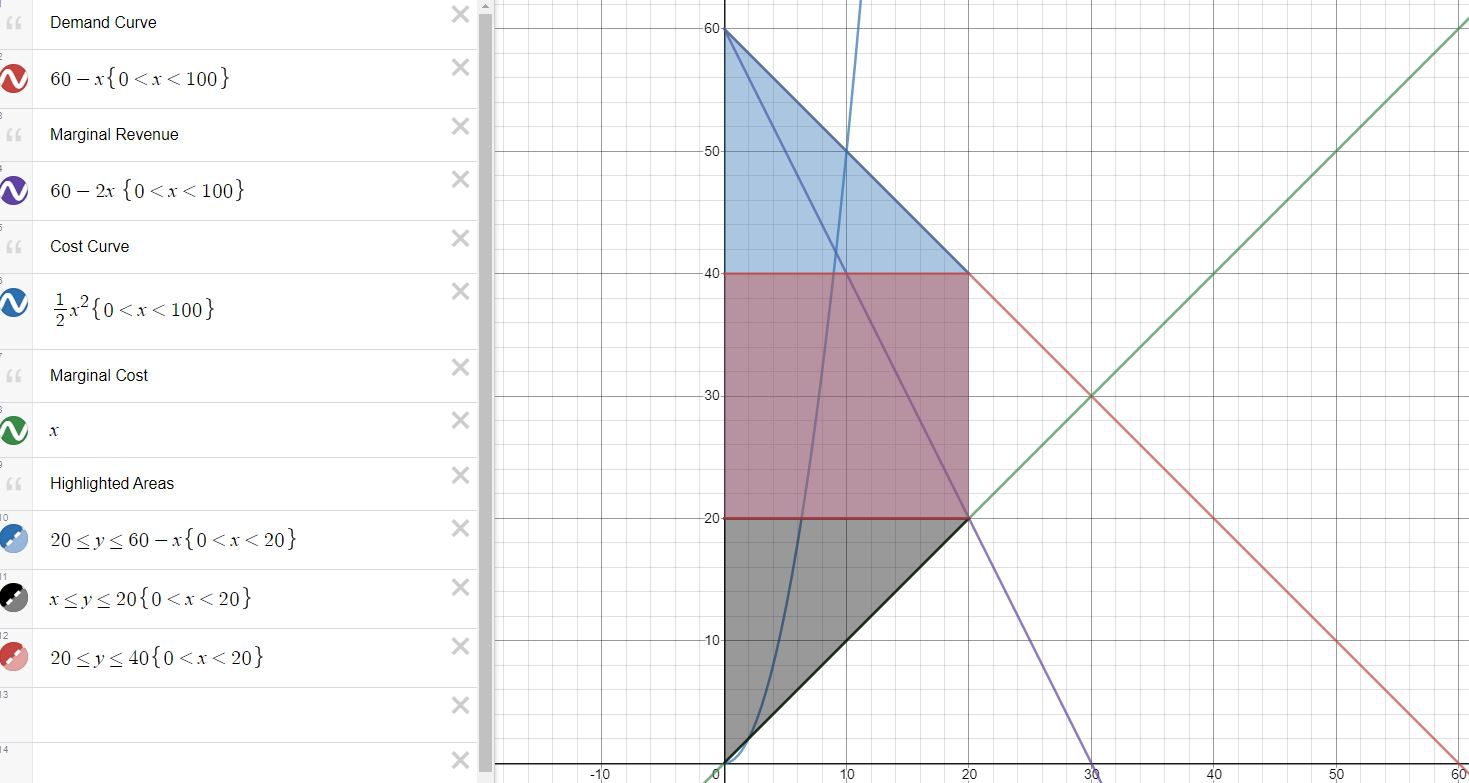
\includegraphics[width=20cm]{./Desmos2.jpg}}
\end{picture}

\end{document}
